\documentclass[letterpaper,10pt]{article}

\usepackage{polski}
\usepackage[utf8]{inputenc}
\usepackage{blindtext}
\usepackage{titling}
\usepackage{setspace}
\usepackage{enumitem}

\usepackage{amsmath}
\usepackage{amssymb}
\usepackage{graphicx}
\usepackage{mathtools}
\usepackage[margin=1.5in]{geometry}
\usepackage{datetime}

%\textwidth=8in \textheight=9in 
%\oddsidemargin=0.5in
%\topmargin=-1in

\author{Paweł Lipkowski}
\title{Zadania świąteczne}
\date{\today} % use \date{\today} or comment this line to have a current date

%\frenchspacing

\DeclareMathOperator{\Q}{\mathbb{Q}}
\newcommand{\R}{\mathbb{R}}
\newcommand{\N}{\mathbb{N}}

\newtheorem{tw}{Twierdzenie}
\newtheorem{lem}{Lemat}
\newtheorem{wn}{Wniosek}
\newtheorem{fakt}{Fakt}
\newtheorem{uw}{Uwaga}
\newtheorem{defin}{Definicja}
\newtheorem{prz}{Przykład}
\newtheorem{zad}{Zadanie}
\newenvironment{dow}{\par \noindent \emph{Dowód.\ }}{\hfill $\Box$ \par}

\newcommand{\tytul}[1]{%
	\begin{center}%
	\LARGE\textbf{#1}%
	\end{center}%
}

\usepackage{eso-pic}
\newcommand\BackgroundPic{%
\put(0,0){%
\parbox[b][\paperheight]{\paperwidth}{%
\vfill
\centering
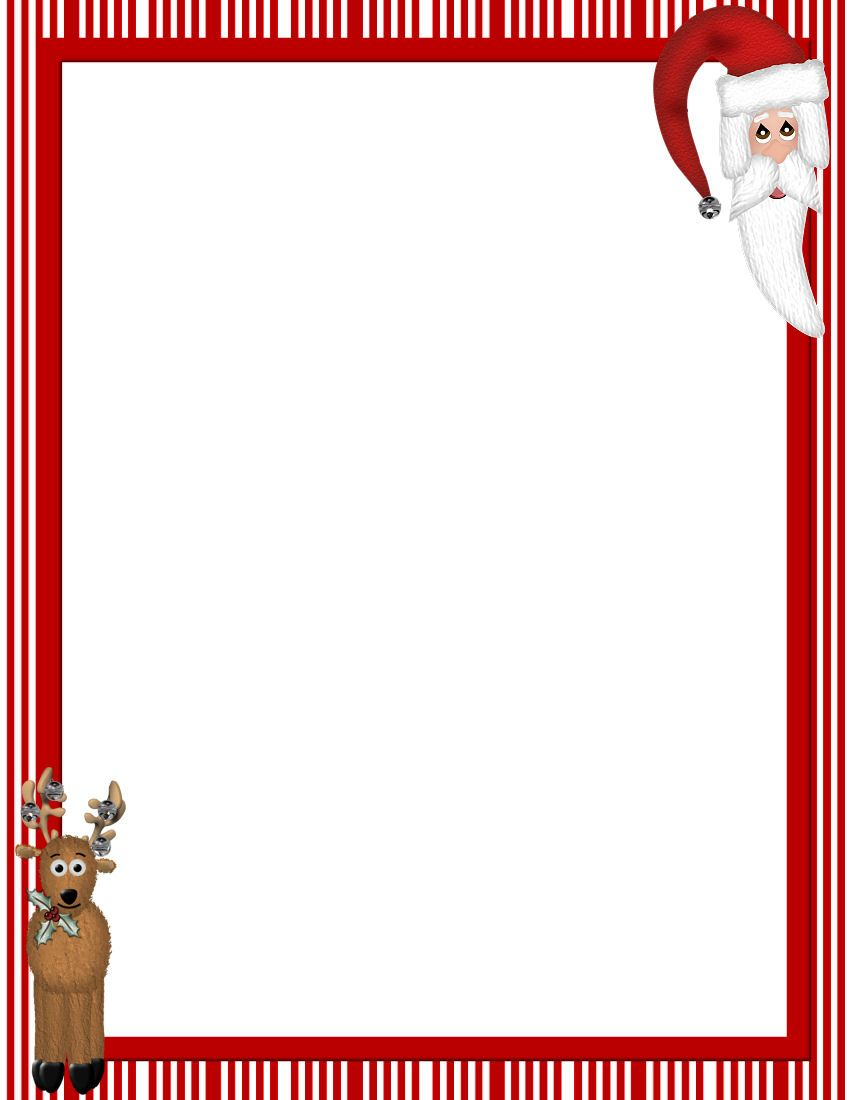
\includegraphics[width=\paperwidth,height=\paperheight,%
keepaspectratio]{tlo.jpg}%
\vfill
}}}

\begin{document}
    \AddToShipoutPicture{\BackgroundPic}
    \begin{tabular}{l p{2.5in}}
		\textbf{Data:}  & \thedate \\
        \textbf{Autor:} & \theauthor \\
    \end{tabular}

    \begin{center}
        \tytul{\thetitle}
    \end{center}
    
    ~
    
    \setstretch{1.25}
    
    \begin{zad}
        Święty Mikołaj ma stajnię pełną reniferów. Przewodniczy owym reniferom czerwononosy Rudolf. Rudolf $\frac{1}{3}$ swojego dnia spędza na spaniu, 
        a ćwiczy dziennie przez czas dłuższy o 2 godziny od czasu na spanie. Połowę pozostałego czasu Rudolf spędza na spędzaniu czasu ze swoją przyjaciółką. 
        Ile to godzin? 
    \end{zad}

    \begin{figure}[h!]
		\centering
  		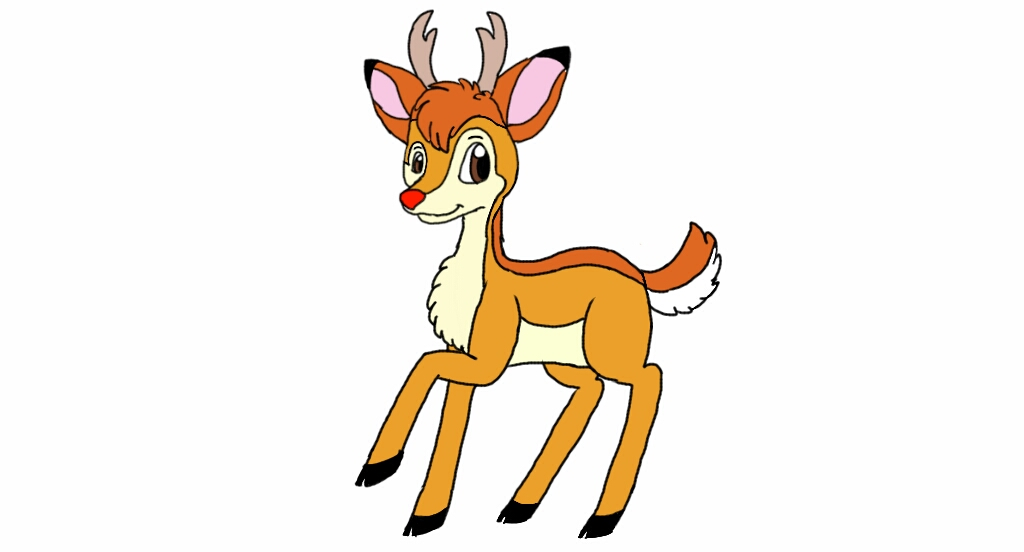
\includegraphics[height=1.5in]{rudolph.jpg}
	\end{figure}

    \begin{zad}
        Sanie Świętego Mikołaja mają wymiary przestrzeni załadunkowej 2m $\times$ 4m. Prezenty są pakowane w paczkach o wymiarach 50cm $\times$ 50cm. 
        Święty Mikołaj przy każdej podróży ładuje 3 warstwy paczek prezentów na sanie, ponadto~każda warstwa paczek wypełnia przestrzeń załadunkową na szerokość i długość.
        Zakładając, że na~Kaszubach mieszka 660~tysięcy~ludzi, ile Święty Mikołaj odbędzie podróży, aby dostarczyć po jednym prezencie dla~każdego Kaszuby?
    \end{zad}

    \begin{figure}[h!]
		\centering
  		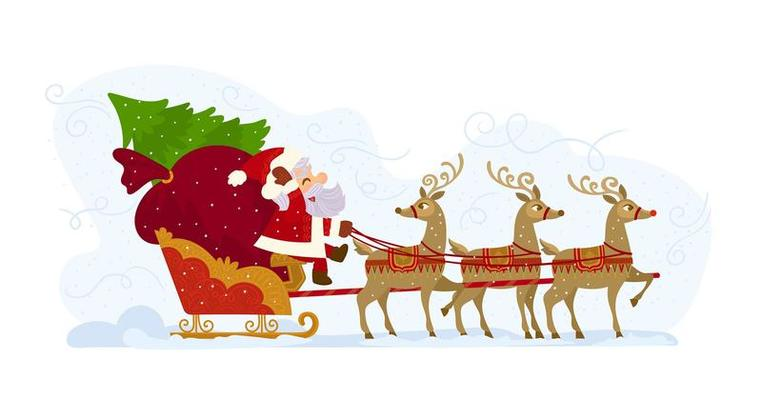
\includegraphics[height=1.5in]{sanie.jpg}
    \end{figure}
    
    \newpage

    ~

    ~

    ~

    \begin{zad}
        Filip chce bardzo odwiedzić Świętego Mikołaja. 
        Postanowił wyruszyć promem z Gdańska do~Helsinek, który wyruszył w~rejs 23~grudnia o~godzinie~15:21. 
        Prom przybył do~Helsinek po~11 godzinach i~38~minutach rejsu. % o 2:59
        Następnie po 41 minutach czekania w~Helsinkach % 3:40 
        wsiadł na dworcu kolejowym do~pociągu, który przez pół~doby wiózł~go do~Rovaniemi, gdzie mieszka Święty Mikołaj. 
        Święty Mikołaj rozpoczyna swoją wigilijną podróż o~16:00. Czy Filip zdąży spotkać~się z~nim?
    \end{zad}

    \begin{figure}[h!]
		\centering
  		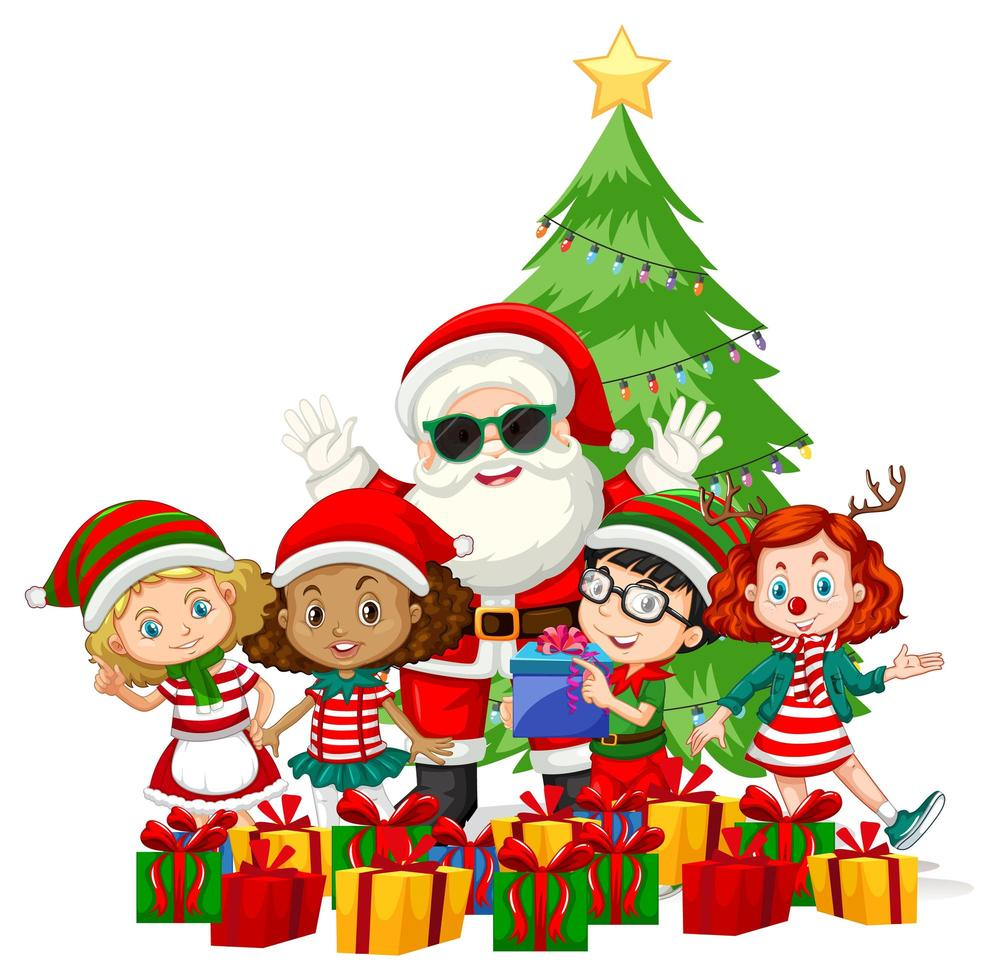
\includegraphics[height=1.5in]{mikolaj1.jpg}
    \end{figure}

    \begin{zad}
        Józef i Maria wędrowali z Nazaretu do Betlejem, gdzie doszło do narodzin Jezusa Chrystusa. 
        Między Nazaretem a Betlejem jest 130 km dystansu, wybierając najkrótszą drogę przez Szechem, Beit El i Jerozolimę.
        Józef i Maria szli pieszo izraelskimi drogami ze średnią prędkością $2 \frac{km}{h}$, robiąc co 15 km przerwy trwające godzinę.
        Ponadto w wyżej wymienionych miastach (Szechem, Beit El, Jerozolima) oboje zrobili po odpoczynku 12-godzinnym.
        \begin{enumerate}[label=\alph*)]
            \item Ile dni trwała podróż?
            \item Przyjmując, że Jezus sie urodził 25 grudnia o północy, to którego dnia kalendarzowego Józef i Maria rozpoczęli podróż?
        \end{enumerate}
    \end{zad}

    \begin{figure}[h!]
		\centering
  		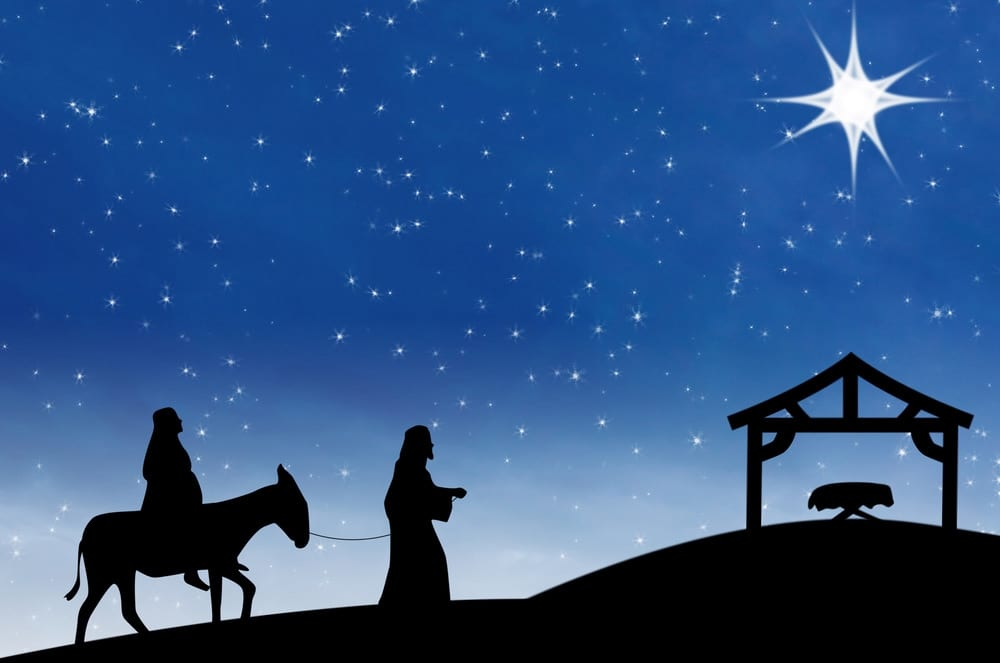
\includegraphics[height=1.5in]{idase2.jpg}
    \end{figure}

\end{document}